% Publication-quality diagram for Hierarchical Ensemble Architecture

\documentclass{article}
\usepackage[a3paper,landscape,margin=1.5cm]{geometry} % Use A3, landscape, larger margin
\usepackage{tikz}
\usetikzlibrary{shapes.geometric, arrows.meta, positioning, calc, decorations.pathreplacing}
\pagestyle{empty}

\definecolor{inputblue}{RGB}{102,194,255}
\definecolor{modelgray}{RGB}{200,200,200}
\definecolor{metapurple}{RGB}{178,102,255}
\definecolor{probgreen}{RGB}{153,221,153}
\definecolor{outputyellow}{RGB}{255,255,153}
\definecolor{filterred}{RGB}{220,50,47}
\definecolor{concatgray}{RGB}{120,120,120}

\begin{document}
\sffamily
\begin{center}
\parbox{\textwidth}{
    \centering
    \textbf{\fontsize{18}{20}\selectfont Hierarchical Ensemble Architecture}
}
\vspace{2em}

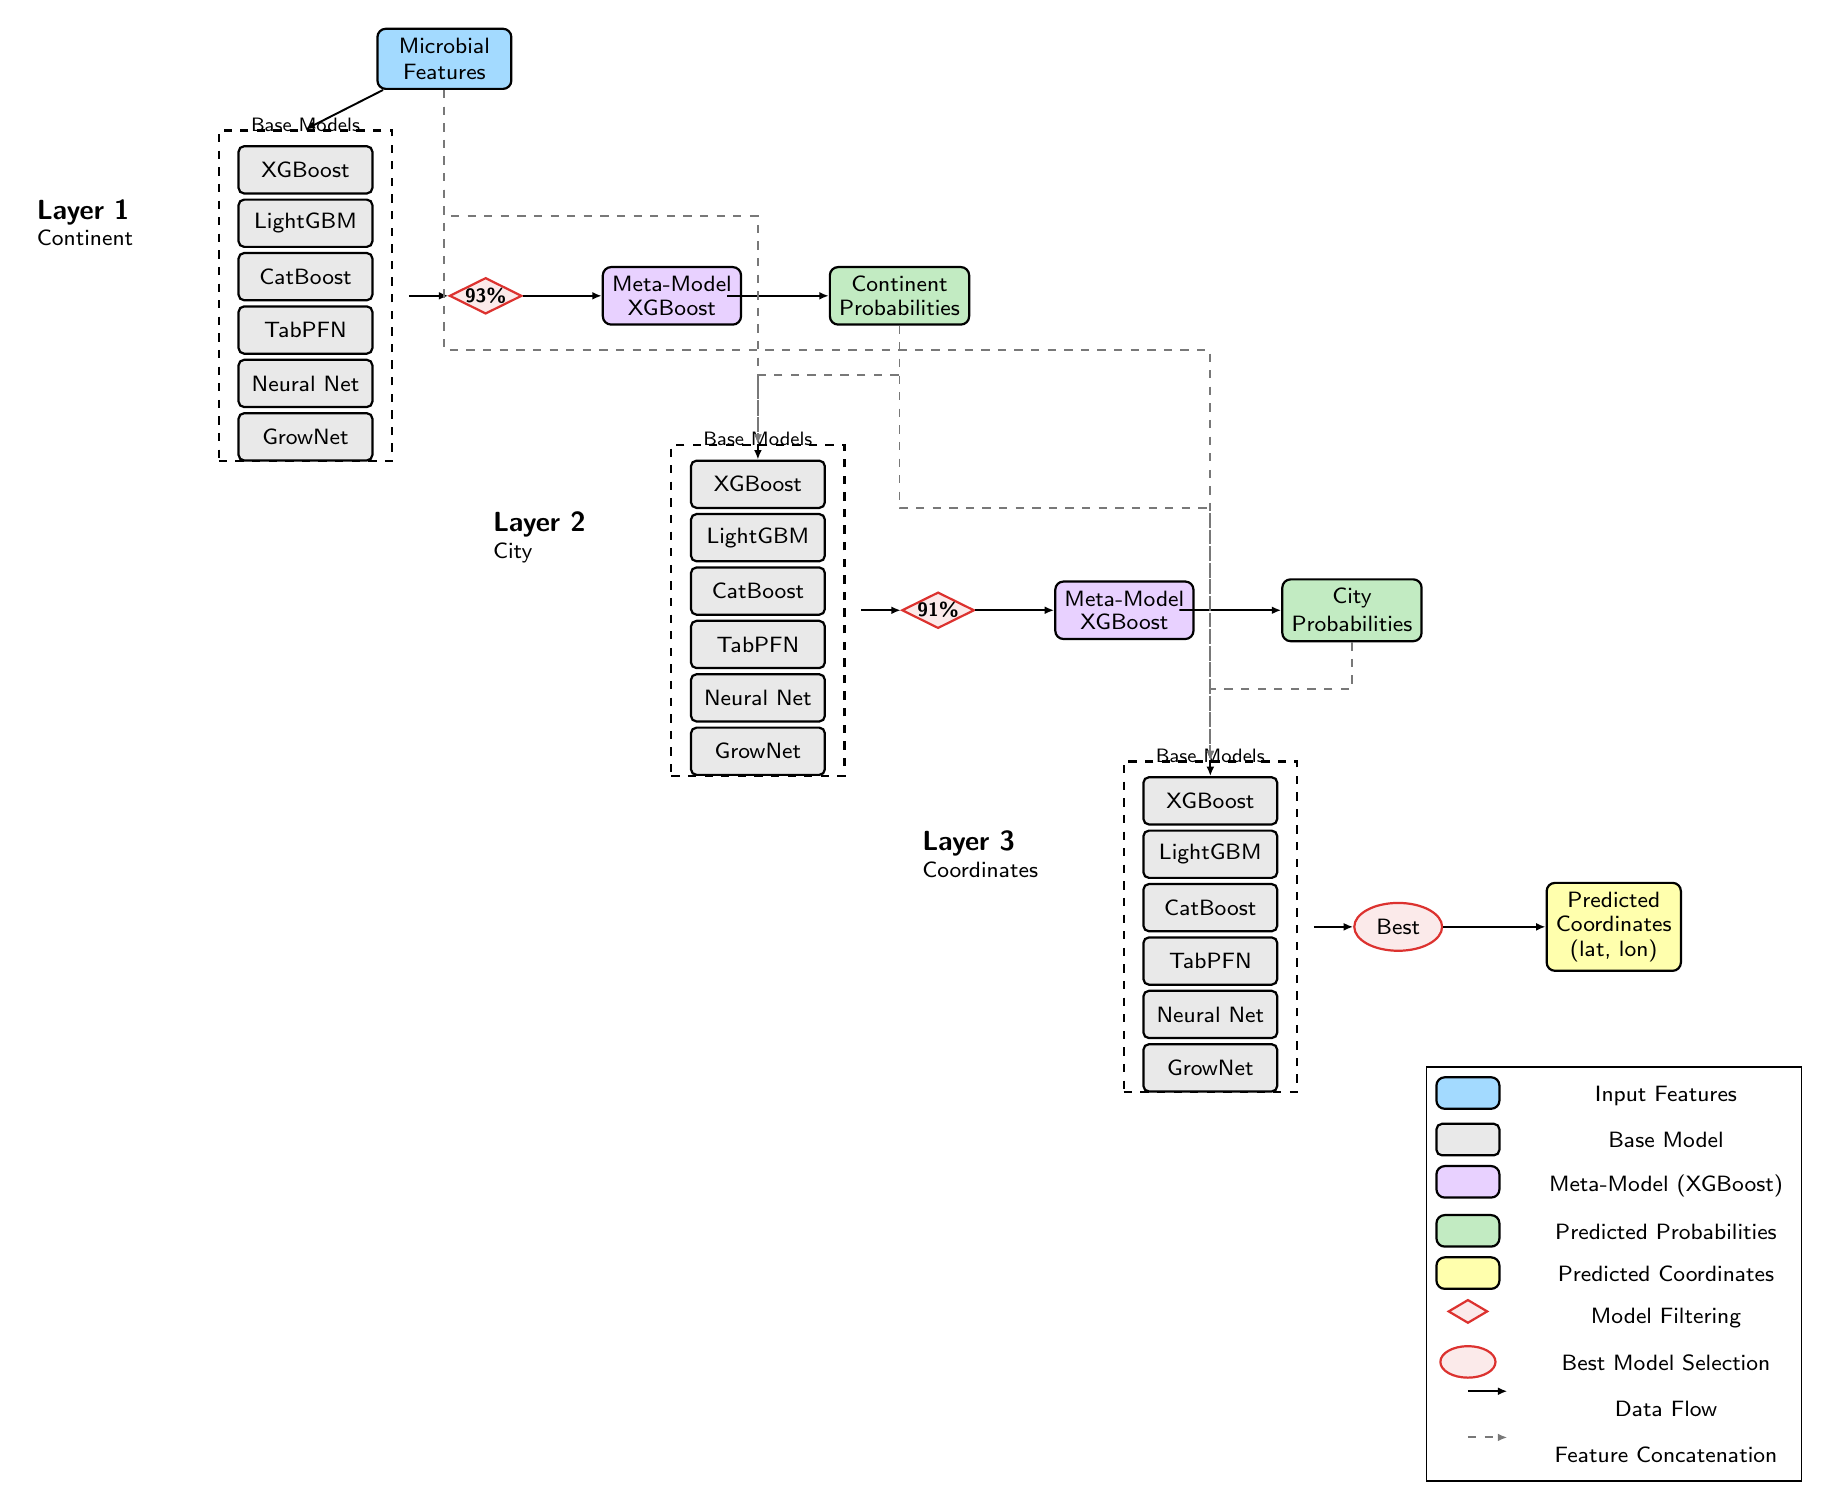
\begin{tikzpicture}[
    node distance=1.1cm and 1.1cm,
    every node/.style={font=\sffamily\footnotesize},
    input/.style={rectangle, rounded corners=3pt, draw=black, fill=inputblue!60, minimum width=1.7cm, minimum height=0.6cm, thick, align=center},
    base/.style={rectangle, rounded corners=2pt, draw=black, fill=modelgray!40, minimum width=1.7cm, minimum height=0.6cm, thick, align=center},
    basegroup/.style={rectangle, draw=black, dashed, minimum width=2.2cm, minimum height=4.2cm, thick, fill=none},
    meta/.style={rectangle, rounded corners=3pt, draw=black, fill=metapurple!30, minimum width=1.5cm, minimum height=0.6cm, thick, align=center},
    prob/.style={rectangle, rounded corners=3pt, draw=black, fill=probgreen!60, minimum width=1.4cm, minimum height=0.5cm, thick, align=center},
    output/.style={rectangle, rounded corners=3pt, draw=black, fill=outputyellow!80, minimum width=1.5cm, minimum height=0.6cm, thick, align=center},
    filter/.style={diamond, aspect=2, draw=filterred, fill=filterred!10, minimum width=0.7cm, minimum height=0.4cm, thick, inner sep=0pt, align=center},
    select/.style={ellipse, draw=filterred, fill=filterred!10, minimum width=0.8cm, minimum height=0.5cm, thick, align=center},
    arrow/.style={very thick, -{Latex[length=1.2mm,width=1mm]}, line width=0.7pt},
    concat/.style={arrow, color=concatgray, dashed},
    legend/.style={rectangle, draw=none, fill=none, font=\footnotesize}
]

% Input node
\node[input] (input) {Microbial\\Features};

% Layer 1: Grouped base models
\node[basegroup, below left=0.5cm and 0.9cm of input, anchor=north] (basegroup1) {};
\node[base, anchor=north, minimum width=1.7cm, minimum height=0.6cm] (xgb1) at ([yshift=-0.2cm]basegroup1.north) {XGBoost};
\node[base, below=0.05cm of xgb1] (lgb1) {LightGBM};
\node[base, below=0.05cm of lgb1] (cat1) {CatBoost};
\node[base, below=0.05cm of cat1] (tabpfn1) {TabPFN};
\node[base, below=0.05cm of tabpfn1] (nn1) {Neural Net};
\node[base, below=0.05cm of nn1] (grow1) {GrowNet};
\node[draw=none, fill=none, font=\sffamily\scriptsize, above=0.05cm of xgb1] (base1label) {Base Models};

% Filtering diamond
\node[filter, right=0.7cm of basegroup1] (filter1) {\textbf{\scriptsize 93\%}};

% Meta-model
\node[meta, right=1.0cm of filter1] (meta1) {\shortstack{Meta-Model\\XGBoost}};

% Continent probabilities
\node[prob, right=1.1cm of meta1] (contprob) {\shortstack{Continent\\Probabilities}};

% Layer 2: Grouped base models
\node[basegroup, below left=1.5cm and 0.9cm of contprob, anchor=north] (basegroup2) {};
\node[base, anchor=north, minimum width=1.7cm, minimum height=0.6cm] (xgb2) at ([yshift=-0.2cm]basegroup2.north) {XGBoost};
\node[base, below=0.05cm of xgb2] (lgb2) {LightGBM};
\node[base, below=0.05cm of lgb2] (cat2) {CatBoost};
\node[base, below=0.05cm of cat2] (tabpfn2) {TabPFN};
\node[base, below=0.05cm of tabpfn2] (nn2) {Neural Net};
\node[base, below=0.05cm of nn2] (grow2) {GrowNet};
\node[draw=none, fill=none, font=\sffamily\scriptsize, above=0.05cm of xgb2] (base2label) {Base Models};

% Filtering diamond
\node[filter, right=0.7cm of basegroup2] (filter2) {\textbf{\scriptsize 91\%}};

% Meta-model
\node[meta, right=1.0cm of filter2] (meta2) {\shortstack{Meta-Model\\XGBoost}};

% City probabilities
\node[prob, right=1.1cm of meta2] (cityprob) {\shortstack{City\\Probabilities}};

% Layer 3: Grouped base models
\node[basegroup, below left=1.5cm and 0.9cm of cityprob, anchor=north] (basegroup3) {};
\node[base, anchor=north, minimum width=1.7cm, minimum height=0.6cm] (xgb3) at ([yshift=-0.2cm]basegroup3.north) {XGBoost};
\node[base, below=0.05cm of xgb3] (lgb3) {LightGBM};
\node[base, below=0.05cm of lgb3] (cat3) {CatBoost};
\node[base, below=0.05cm of cat3] (tabpfn3) {TabPFN};
\node[base, below=0.05cm of tabpfn3] (nn3) {Neural Net};
\node[base, below=0.05cm of nn3] (grow3) {GrowNet};
\node[draw=none, fill=none, font=\sffamily\scriptsize, above=0.05cm of xgb3] (base3label) {Base Models};

% Selection ellipse (instead of star)
\node[select, right=0.7cm of basegroup3] (select3) {Best};

% Output coordinates
\node[output, right=1.3cm of select3] (coordout) {\shortstack{Predicted\\Coordinates\\(lat, lon)}};

% --- Arrows and connections (shorten horizontal arrows) ---

% Input to base models (single arrow to group)
\draw[arrow] (input) -- ([yshift=0.0cm]basegroup1.north);

% Base models to filter (single arrow from group)
\draw[arrow] ([xshift=0.2cm]basegroup1.east) -- (filter1);

% Filter to meta-model (Layer 1)
\draw[arrow] (filter1) -- ++(0.7,0) |- (meta1);

% Meta-model to continent probabilities
\draw[arrow] (meta1) -- ++(0.7,0) |- (contprob);

% Feature concatenation for city layer (shorter)
\draw[concat] (input) -- ++(0,-2.0) -| ([yshift=0.0cm]basegroup2.north);
\draw[concat] (contprob) -- ++(0,-1.0) -| ([yshift=0.0cm]basegroup2.north);

% Input to city base models (single arrow to group)
\draw[arrow] ([yshift=0.0cm]basegroup2.north) -- (xgb2);

% Base models to filter (single arrow from group)
\draw[arrow] ([xshift=0.2cm]basegroup2.east) -- (filter2);

% Filter to meta-model (Layer 2)
\draw[arrow] (filter2) -- ++(0.7,0) |- (meta2);

% Meta-model to city probabilities
\draw[arrow] (meta2) -- ++(0.7,0) |- (cityprob);

% Feature concatenation for coordinate layer (shorter)
\draw[concat] (input) -- ++(0,-3.7) -| ([yshift=0.0cm]basegroup3.north);
\draw[concat] (contprob) -- ++(0,-2.7) -| ([yshift=0.0cm]basegroup3.north);
\draw[concat] (cityprob) -- ++(0,-1.0) -| ([yshift=0.0cm]basegroup3.north);

% Input to coordinate base models (single arrow to group)
\draw[arrow] ([yshift=0.0cm]basegroup3.north) -- (xgb3);

% All coordinate base models to selection (single arrow from group)
\draw[arrow] ([xshift=0.2cm]basegroup3.east) -- (select3);

% Selection to output
\draw[arrow] (select3) -- ++(0.7,0) |- (coordout);

% --- Layer labels ---
\node[align=left, left=1.2cm of lgb1] (l1) {\textbf{\normalsize Layer 1}\\Continent};
\node[align=left, left=1.2cm of lgb2] (l2) {\textbf{\normalsize Layer 2}\\City};
\node[align=left, left=1.2cm of lgb3] (l3) {\textbf{\normalsize Layer 3}\\Coordinates};

% --- Legend ---
\matrix[draw, below=1.2cm of coordout, column sep=0.4cm, row sep=0.1cm, font=\sffamily\scriptsize] (legend) {
    \node[input, minimum width=0.8cm, minimum height=0.4cm] {}; & \node {Input Features}; \\
    \node[base, minimum width=0.8cm, minimum height=0.4cm] {}; & \node {Base Model}; \\
    \node[meta, minimum width=0.8cm, minimum height=0.4cm] {}; & \node {Meta-Model (XGBoost)}; \\
    \node[prob, minimum width=0.8cm, minimum height=0.4cm] {}; & \node {Predicted Probabilities}; \\
    \node[output, minimum width=0.8cm, minimum height=0.4cm] {}; & \node {Predicted Coordinates}; \\
    \node[filter, minimum width=0.5cm, minimum height=0.3cm] {}; & \node {Model Filtering}; \\
    \node[select, minimum width=0.7cm, minimum height=0.4cm] {}; & \node {Best Model Selection}; \\
    \draw[arrow] (0,0) -- (0.5,0); & \node {Data Flow}; \\
    \draw[concat] (0,0) -- (0.5,0); & \node {Feature Concatenation}; \\
};

\end{tikzpicture}

\vspace*{0.5em}

\end{center}
\end{document}
